\documentclass[11pt]{article}
\usepackage[spanish]{babel} % Paquete de español
\usepackage{natbib}
\usepackage{url}
\usepackage[utf8]{inputenc} % Codificación
\usepackage{amsmath}
\usepackage{graphicx}
\graphicspath{{images/}} % Carpeta en la cual se van a buscar las imagenes
\usepackage{subfigure}	% Permite la Inclusión de subfiguras
%\usepackage{parskip} % Borrar identación de parrafos.
\setlength{\parskip}{3mm} % Longitud del espaciado entre parrafos
\usepackage[hidelinks]{hyperref} % Referencias (links)
\usepackage{fancyhdr}
\usepackage{vmargin}
\setpapersize{A4} % Formato del papel - A4
\setmarginsrb{3 cm}{2.5 cm}{3 cm}{2.5 cm}{1 cm}{1.5 cm}{1 cm}{1.5 cm} % Margenes
\usepackage{paralist} % Permite un mayor control sobre las listas
\usepackage{textcomp,marvosym,pifont} % Generación de símbolos especiales

%%%%%%%%%%%%%%%%%%%%%%%%%%%%%%%%%%%%%%%%%%%%%%%%%%%%%%%%%%%%%%%%%%%%%%%%%%%%%%%%%%%%%%%%%
% Insertar código en la memoria:
% A partir de 'Listados de código cómodos y resultones con listings' de David Villa
% http://crysol.org/es/node/909

\usepackage{color}
\definecolor{gray97}{gray}{.97}
\definecolor{gray75}{gray}{.75}
\definecolor{gray45}{gray}{.45}

\usepackage{listings}
\lstset{ frame=Ltb,
	framerule=0pt,
	aboveskip=0.5cm,
	framextopmargin=3pt,
	framexbottommargin=3pt,
	framexleftmargin=0.4cm,
	framesep=0pt,
	rulesep=.4pt,
	backgroundcolor=\color{gray97},
	rulesepcolor=\color{black},
	texcl=true,
	%
	stringstyle=\ttfamily,
	showstringspaces = false,
	basicstyle=\small\ttfamily,
	commentstyle=\color{gray45},
	keywordstyle=\bfseries,
	%
	numbers=left,
	numbersep=15pt,
	numberstyle=\tiny,
	numberfirstline = false,
	breaklines=true,
}

% minimizar fragmentado de listados
\lstnewenvironment{listing}[1][]
{\lstset{#1}\pagebreak[0]}{\pagebreak[0]}

\lstdefinestyle{consola}
{basicstyle=\scriptsize\bf\ttfamily,
	backgroundcolor=\color{gray75},
}

\lstdefinestyle{C}
{language=C,
}
%%%%%%%%%%%%%%%%%%%%%%%%%%%%%%%%%%%%%%%%%%%%%%%%%%%%%%%%%%%%%%%%%%%%%%%%%%%%%%%%%%%%%%%%%

\renewcommand{\lstlistingname}{Listado} % Renombrar listados para que aparezcan en español.
\usepackage{float} % Permite usar H en las figuras, de manera que se coloquen en la posición exacta en la que están en el código.


% Añade un comando para crear indicaciones de pulsación de teclas
\usepackage{tikz} % Paquete especializado en gráficos
\usetikzlibrary{shadows} % Necesario para poder crear nuevo comando de indicación de pulsación de tecla.
\newcommand*\tecla[1]{%   
	\tikz[baseline=(key.base)]
	\node[%
	draw,
	fill=white,
	drop shadow={shadow xshift=0.25ex,shadow yshift=-0.25ex,fill=black,opacity=0.75},
	rectangle,
	rounded corners=2pt,
	inner sep=1pt,
	line width=0.5pt,
	font=\scriptsize\sffamily
	](key) {#1\strut}
	;
}

%%%%%%%%%%%%%%%%%%%%%%%%%%%%%%%%%%%%%%%%%%%%%%%%%%%%%%%%%%%%%%%%%%%%%%%%%%%%%%%%%%%%%%%%%
% Principales variables del documento

\title{Titulo de la práctica}							% Titulo
\author{José~Ángel~Martín~Baos}							% Autor
\date{\today}											% Fecha

\makeatletter
\let\thetitle\@title
\let\theauthor\@author
\let\thedate\@date
\makeatother

\pagestyle{fancy}
\fancyhf{}
\rhead{\theauthor}
\lhead{\thetitle}
\cfoot{\thepage}

\begin{document}

%%%%%%%%%%%%%%%%%%%%%%%%%%%%%%%%%%%%%%%%%%%%%%%%%%%%%%%%%%%%%%%%%%%%%%%%%%%%%%%%%%%%%%%%%
% Portada

\begin{titlepage}
	\centering
    
\includegraphics[scale = 0.40]{uclm_logo.pdf}\\[1.0 cm]	% Logo de la universidad
    
\includegraphics[scale = 0.25]{esi.pdf}\\[1.0 cm]
    \textsc{\LARGE Universidad de Castilla-La Mancha}\\[0.5 cm]	% Nombre de la universidad
    \textsc{\LARGE Escuela Superior de Informática}\\[2.0 cm]
	\textsc{\Large Asignatura}\\[0.5 cm]				% Asignatura
	\textsc{\large 3º Ingeniería de Computadores}\\[0.5 cm]						% Curso
	\rule{\linewidth}{0.2 mm} \\[0.4 cm]
	{ \huge \bfseries \thetitle}\\
	\rule{\linewidth}{0.2 mm} \\[1.5 cm]
	
	\begin{minipage}{0.4\textwidth}
		\begin{flushleft} \large
			\emph{Autor:}\\
			\theauthor
			\end{flushleft}
			\end{minipage}~
			\begin{minipage}{0.4\textwidth}
			\begin{flushright} \large
			\emph{Fecha:} \\
			\thedate
		\end{flushright}
	\end{minipage}\\[1.5 cm]
 
	\vfill
	
\end{titlepage}

%%%%%%%%%%%%%%%%%%%%%%%%%%%%%%%%%%%%%%%%%%%%%%%%%%%%%%%%%%%%%%%%%%%%%%%%%%%%%%%%%%%%%%%%%
% Indice

\tableofcontents
\pagebreak

%%%%%%%%%%%%%%%%%%%%%%%%%%%%%%%%%%%%%%%%%%%%%%%%%%%%%%%%%%%%%%%%%%%%%%%%%%%%%%%%%%%%%%%%%

\section{Introducción}
Este es un ejemplo de una plantilla hecha con \LaTeX para la realización de trabajos y entregas de laboratorio de la ESI (Escuela Superior de Informática) de Ciudad Real, Universidad de Castilla-La Mancha. Esta plantilla ha sido creada por \href{https://github.com/JoseAngelMartinB}{José Ángel Martín Baos}.


\begin{figure}[H] 
	\centering
	
\includegraphics[angle=0]{licencia}
%	\caption{Licencia Creative Commons}
%	\label{fig:licencia}
\end{figure}	
Esta obra está bajo una licencia de Creative Commons Reconocimento-CompartirIgual 4.0 Internacional.
\href{https://creativecommons.org/licenses/by-sa/4.0/}{https://creativecommons.org/licenses/by-sa/4.0/}


\section{Ejemplo de códigos e imágenes}
En está sección se explica brevemente como usar algunas características básicas de \LaTeX como pueden ser \textbf{texto en negrita}, \emph{enfatizado}, \textit{cursiva}, \underline{subrayado}, \textsc{o versalitas}.

También se pueden insertar códigos (listados) de la siguiente forma:
\lstinputlisting[style=C,
caption={Ejemplo de un listado de código},
label={lst:HolaMundo},
firstline=1]{code/hola_mundo.c}

Podemos hacer referencia en cualquier momento a Listado \ref{lst:HolaMundo}

Para insertar imágenes (figuras) podemos usar los siguientes comandos, ya sea una imagen individual o dos subimágenes. También podemos hacer referencia a dichas imágenes: Figura \ref{fig:PlazaCR} o Figura \ref{fig:ESI1}.

% Una imagen
\begin{figure}[H] %H --> Obliga a que la imagen se coloque en el lugar exacto
	\centering
	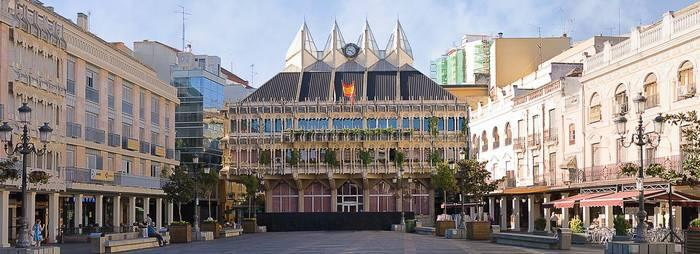
\includegraphics[width=1\linewidth,angle=0]{PlazaCR}
	\caption{Plaza de Ciudad Real}
	\label{fig:PlazaCR}
\end{figure}	

% Dos subimagenes
\begin{figure}[htb]
	\centering
	\subfigure[Imagen de la fachada de la ESI]{
		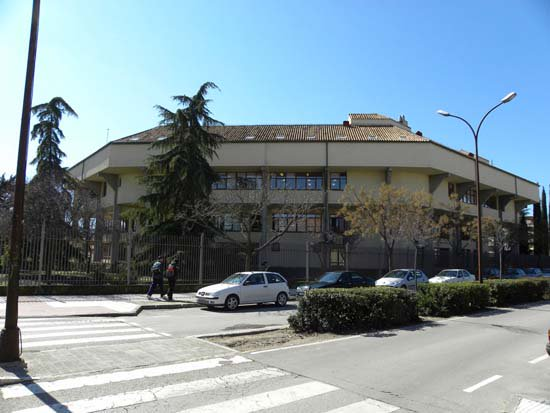
\includegraphics[width=7cm]{ESI2}
		\label{fig:ESI1}
	}
	\subfigure[Imagen de la ESI]{
		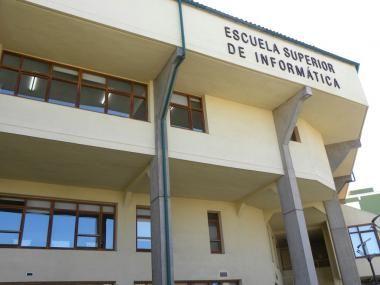
\includegraphics[width=7cm]{ESI1}
		\label{fig:ESI2}
	}
	\caption{Imágenes que muestran la ESI}
	\label{fig:ESI}
\end{figure}

Ademas de lo anterior, podemos insertar comandos de consla de la siguiente forma:
\begin{listing}[style=consola, numbers=none]
$ uname -a
Linux droideka 4.4.0-66-generic #87-Ubuntu SMP Fri Mar 3 15:29:05 UTC 2017 x86_64 x86_64 x86_64 GNU/Linux
\end{listing} %$

También podemos de la forma: \texttt{uname -a}.

Por último, para recrear la pulsación de un botón podemos usar: \tecla{Ctrl+C}


\section{Ejemplo de listados y referencias}

En este ejemplo vamos a mostrar el uso de un listado compacto.

\begin{compactitem}
	\item Item 1
	\item Item 2
	\item Item 3
	\item Item 4
\end{compactitem}

A parte de las listas, también podemos citar libros o artículos mediante el comando cite. \cite{Kottwitz2011} \cite{Martin2017} \cite{Salido2011}

%%%%%%%%%%%%%%%%%%%%%%%%%%%%%%%%%%%%%%%%%%%
% BIBLIOGRAPHY
%%%%%%%%%%%%%%%%%%%%%%%%%%%%%%%%%%%%%%%%%%%
\newpage
\bibliography{biblist}
\bibliographystyle{plain}

\end{document}